\chapter{Tradução de ROBO para CSP}
A Seção 3.1 descreve como foi realizado o processo de tradução automático de ROBO para CSP através do framework Spoofax. Desde a fase inicial da definição da gramática até a geração de código.

\section{Processo de Tradução Automática}

\subsection{Ferramentas e Ambiente de Programação}
O desenvolvimento de um compilador exige uma preparação bem elaborada de todo um ambiente de programação. No caso deste trabalho, foi necessário o uso do ambiente de programação Eclipse juntamente com um plugin do Spoofax. O qual foi essencial para o desenvolvimento da abordagem de tradução automática. O plugin tem todas as depedências para a geração de Árvore de Análise Sintática e transformação de código.

\section{Definição da Linguagem ROBO com Spoofax}
Nesta Seção veremos como ocorrreu todo o processo de definição da linguagem ROBO usando o framework Spoofax, o que inclui a definição da sintaxe e transformação da linguagem, resultando em código CSP.
\subsection{Definição da Sintaxe}
Essa é a etapa inicial para a construção do compilador, na qual devemos primeiro definir todos os aspectos sintáticos da linguagem de programação utilizada no ambiente RoboMind. Ou seja, essa etapa deverá ser capaz de considerar os programas escritos na linguagem ROBO e assegurá-los que estão sintaticamente corretos. Para a definição da gramática livre de contexto de ROBO foi utilizado o formalismo SDF3, como já explicado no Capítulo \ref{chap:cap2}. Além de definir a gramática, SDF3 também foi utilizado para definir a sintaxe lexical, como por exemplo, palavras reservadas de ROBO. O principal objetivo dessa etapa a geração de uma Árvore Sintática Abstrata (\textit{Abstract Syntax Tree - AST}, em inglês) dos programas ROBO. Esse produto resultante é de extrema importância para a geração de código CSP através do Stratego.

É importante saber que a linguagem ROBO possui algumas características que a difere das linguagens de programação comuns, uma vez que se trata de uma DSL, com um objetivo bem definido. Abaixo estão listadas algumas das principais características de ROBO:

\begin{itemize}
    \item Funções booleanas predefinidas para detecção de obstáculos ou objetos ao redor do robô, por exemplo \textit{frontIsObstacle}, para verificar se há obstáculo na frente do robô ou \textit{frontIsClear}, para verificar se a frente do robô está livre de quaisquer objetos.
    \item Funções predefinidas para a movimentação do robô, como por exemplo \textit{forward(n)}, para movimentar para frente ou \textit{backward(n)}, para movimentar para trás.
    \item Variáveis globais.
    \item Procedimentos parametrizados e não parametrizados.
    \item Estruturas condicionais e de repetição, assim como na maioria das linguagens de programação.
    \item Expressões aritméticas com valores inteiros.
\end{itemize}

Para exemplificar todo o processo de compilação, definimos um exemplo de programa em ROBO que resolve um problema específico. O problema definido foi o ``Contando Caixas'', proposto por RoboLab-FURB\ref{add-ref} e adaptamos para esta pesquisa. O objetivo desse problema é propor uma solução para a simulação de um robô capaz de contar caixas espalhadas por diferentes cenários. O problema foi alterado para que exista um parâmetro que determina o lado no qual o robô deverá contar, sendo lado esquerdo ou direito. Na Figura \ref{fig:map} é mostrado um mapa utilizado para a simulação do problema em questão. Nele é possível ver um robô e algumas caixas, duas na linha superior e três na linha inferior. Na figura foi adicionado um ``X'' para indicar a posição final que o robô deverá parar após a execução do programa. Para exemplificar uma simulação, considere que o lado direito foi escolhido como parâmetro, desse modo, o robô deverá percorrer em linha reta contando as caixas à sua direita e ao chegar na posição final mostrará o resultado 3, caso o parâmetro fosse o lado esquerdo, a quantidade de caixas contadas pelo robô seria 2.

\begin{figure}[h]
\centering
\caption{Exemplo de Mapa usado no RoboMind}
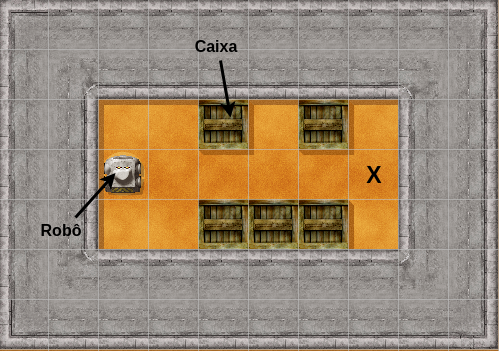
\includegraphics[height=7cm]{figuras/map2.png}
\fonte{O autor}
\label{fig:map}
\end{figure}

Na Figura \ref{fig:roboprogram} está disposto o código de um programa que resolve o problema da contagem de caixas. Esse programa possui duas variáveis globais: (a) \textit{countBoxes}, que é responsável por amazenar a quantidade de caixas; e (b) \textit{lookLine}, que é para indicar qual a linha que o robô deve contar as caixas (esquerda ou direita). Também há um procedimento parametrizado chamado \textit{countLine()}, este possui um único parâmetro denominado \textit{side}, o qual indicará o lado que o robô irá analisar. Se o valor passado ao parâmetro for igual a 1, então contará as caixas do lado esquerdo, se for qualquer valor diferente de 1, então contará as caixas do lado direito. O primeiro movimento do robô ocorre através do comando \textit{right} (indicado na linha 16), o qual altera sua orientação em 90 graus à direita. O próximo passo é a execução de um laço pelo comando \textit{repeatWhile}, a repetição ocorre enquanto não houver quaisquer objetos ou paredes na célula à frente do robô. Esse laço é responsável por chamar o procedimento \textit{countLine()} passando o valor da variável \textit{lookLine}, que neste exemplo tem valor 1, ou seja, contará as caixas da linha esquerda, seguindo de um \textit{forward} que move o robô para frente em uma unidade a cada execução do laço. Ao sair dessa estrutura de repetição, o procedimento será executado mais uma vez, com o objetivo de verificar possíveis caixas na última posição do robô e por fim a quantidade de caixas é exibida por meio do comando \textit{show} exibindo o valor armazenado na variável \textit{countBoxes} contendo a quantidade de caixas na linha de interesse. Este exemplo servirá para toda as etapas, desde a geração de uma AST, após a execução do parser, até a geração de código CSP, após a transformação da árvore.

\begin{figure}[h]
\caption{Programa escrito em ROBO}
\lstinputlisting{codes/program1.rob}
\fonte{O autor}
\label{fig:roboprogram}
\end{figure}

O trabalho \cite{nogueira}, como já mencionado, propõe um compilador que contempla a tradução de programas ROBO sem variáveis e procedimentos. No entanto, a gramática definida resulta uma AST é um formato  \texttt{Program(Sequence, Sequence)} similar a uma tupla, sendo assim, uma limitação, o que impossibilitava o uso de funções do framework Spoofax que facilitassem a transformação da árvore, como por exemplo, aplicação de filtros e recolhimento de termos específicos. Sabendo disso, para facilitar o trabalho em cima da árvore, foi necessário reconstruir partes da gramática de modo que a AST gerada tivesse um formato de lista, assim tornando possível o uso das funções nativas do Spoofax. Na Figura \ref{fig:gramatica_antes} tem um trecho da gramática definida no trabalho citado.

\begin{figure}[h]
\caption{Gramática escrita em forma de sequência}
\lstinputlisting[language=Java]{codes/gramatica_antes.sdf3}
\fonte{O autor}
\label{fig:gramatica_antes}
\end{figure}

Já na Figura \ref{fig:gramatica} a gramática foi totalmente reescrita, antes o que era \texttt{Sequence} tornou-se \texttt{Statement} seguido pelo operador * de concatenação. Dessa forma, ao invés do programa iniciar com uma \texttt{Sequence}, a qual também era seguido por uma \texttt{Sequence} precedida de uma \texttt{Instr}. Além dessa mudança, foi adicionado o termo \texttt{Declaration} (linha 6) que possui três tipos: \texttt{Variable}, \texttt{Procedure} e \texttt{ProcParam} (linhas 8, 9 e 12, respectivamente).

\begin{figure}[h]
\caption{Gramática escrita em forma de lista}
\lstinputlisting[language=Java]{codes/gramatica.sdf3}
\fonte{O autor}
\label{fig:gramatica}
\end{figure}

A definição da sintaxe é composta por módulos que podem ser importados e utilizados em outros módulos. Sabendo disso, o compilador de ROBO foi composto por 4 módulos: (1) \textit{Commom}, contendo toda a parte léxica da linguagem, como restrinções e palavras reservadas; (2) \textit{ExpressionsBoolean}, possuindo todas as definições da gramática para expressões booleanas; (3) \textit{ExpressionsMath}, contém a gramática livre de contexto e as prioridades de análise de cálculo matemático; e (4) \textit{Robo2CSP}, este é o módulo principal, pois engloba os demais, além de definir toda a gramática essencial da linguagem ROBO.

Um programa ROBO consiste em uma lista de declarações (\texttt{Statement}) que podem ser do tipo \texttt{Instr} ou \texttt{Declaration}. O tipo \texttt{Instr} contém todas as instruções básicas de ROBO, ou seja, é composta pelos comandos de movimentação, pintura de mapa, caputura de objetos e as estruturas condicionais e de repetição. Já o tipo \texttt{Declaration} é combinado de declarações para variáveis e para a declaração de procedimentos parametrizados e não parametrizados. Assim, está disposto na Figura \ref{fig:gramatica} parte do módulo Robo2CSP, nela estão definidas as produções da linguagem.

A produção \texttt{Statement.Declaration} define três alternativas para o tipo Declaration que estão definidas em três produções separadas, a primeira \texttt{Declaration.Varia\-ble}, para representar as variáveis, a segunda é \texttt{Declaration.Procedure}, para representar os procedimentos não parametrizados e por fim, \texttt{Declaration.ProcParam}, para representar elementos sintáticos de procedimentos parametrizados.

O corpo da produção para variáveis \texttt{<<Identifier> = <Expr>>} define uma declaração do tipo \texttt{Variable} composta de um identificador (\texttt{Identifier}), que é basicamente um texto descrevendo o nome da variável, seguido por um simbolo de igual e terminado por uma expressão que podem ser do tipo booleanas ou matemáticas (indicadas nas linhas 31 e 32 da Figura \ref{fig:gramatica}, respectivamente).

Para os procedimentos há duas produções, a primeira é para os procedimentos não parametrizados (\texttt{<proce\-dure <Identifier>\{ <Statement*> \}>}) que é composto pela palavra reservada \textit{procedure}, seguido por um identificador, que por sua vez é seguido por zero ou mais \texttt{Statement} entre um par de abre-fecha chaves. Já o segundo, para os procedimentos parametrizados, exige uma complexidade maior, uma vez que um procedimento pode ter \textit{n} parâmetros. A diferença do corpo (\texttt{<procedure <Identifier> <Params> \{ <Statement*> \}}) da produção desse tipo para o corpo do procedimento não parametrizado está na existência da produção \texttt{Params} (linha 28 da Figura \ref{fig:gramatica}) logo após o identificador. O corpo de \texttt{Params} é composto por zero ou mais identificadores separados por vírgula dentro dos símbolos de abre-fecha parênteses.

Uma vez definida as produções para declaração de procedimento, agora é necessário a definição de produções para chamada do mesmo. Esta produção está indicada na linha 34 da Figura \ref{fig:gramatica}. Uma chamada de procedimento nada mais é do que um subtipo de \texttt{Instr}, chamado de \texttt{ProcCall}. O corpo desta produção é composto por um identificador seguido pelos parâmetros, os quais são derivados de expressões. Por isso foi definido um novo tipo de produção, chamado de \texttt{ExprParams} que são \textit{n} expressões separadas por vírgula, entre um par de abre-fecha parênteses.

Descrito o passo a passo de como foi definida a gramática da linguagem ROBO. Agora, entra a etapa do \textit{parsing}, ou seja, o compilador consegue ler um programa escrito em ROBO e gerar sua Árvore Sintática Abstrata com todos os elementos do programa de modo estruturado. Consederando o programa ROBO mostrado na Figura \ref{fig:roboprogram}, geramos a sua AST após a execução do \textit{parsing}. A árvore está denotada pelas Figuras \ref{fig:ast1} e \ref{fig:ast2}, a primeira representa o programa, e a segunda representa o contéudo representado por reticências da linha 4 da figura anterior.

\begin{figure}[h]
\centering
\caption{Geração da AST do programa ROBO}
\lstinputlisting[language=Java]{codes/ast2.aterm}
\fonte{O autor}
\label{fig:ast1}
\end{figure}

\begin{figure}[h]
\centering
\caption{Geração de uma AST do procedimento \textit{countLine()}}
\lstinputlisting[language=Java]{codes/ast1.aterm}
\fonte{O autor}
\label{fig:ast2}
\end{figure}

A geração da AST é essencial para a etapa de geração de código através do Stratego. O Stratego precisa de uma uma árvore como entrada em um formato que facilite sua análise, por isso que as ASTs são representadas em um formato textual, como visto anteriormente. Esse formato é denominado de Formato de Termo Anotado (\textit{Annotated Term Format - ATerm, em inglês}) e cada elemento da árvore é chamado de \textit{Term}. Sabendo disso, a próxima Seção descreve o passo a passo de como é realizada a análise da árvore e como foram definidas as regras de compilação para a geração de código CSP em cima dos \textit{ATerms}.

\subsection{Transformação com Stratego}

Essa etapa é a mais importante, em razão de que o resultado deste processo é o código CSP, produto essencial para a verificação dos programas ROBO semanticamente equivalentes à ROBO no verificador de modelos FDR.

O primeiro passo foi definir uma regra em Stratego para manipular os principais termos de um AST. No qual, para cada termo, outras regras são aplicadas, isto é, o conjunto resultante de termos aplicados à uma regra é utilizado pela regra consecutiva. A regra definida na Figura \ref{fig:rules} deve casar com o termo \texttt{Program(T1)}, onde \texttt{T1} é todo o restante da árvore. Assim, todas as demais regras são aplicadas aos termos derivados de \texttt{T1}.

....

\begin{figure}[h]
\centering
\caption{Regra inicial para um programa ROBO}
\lstinputlisting[language=Java]{codes/rules.str}
\fonte{O autor}
\label{fig:rules}
\end{figure}

\begin{figure}[h]
\centering
\caption{Conjunto de regras auxiliares}
\lstinputlisting[language=Java]{codes/rulesAux.str}
\fonte{O autor}
\label{fig:rules2}
\end{figure}
